\documentclass{article}

\usepackage[margin=1in]{geometry} 
\usepackage{amsmath,amsthm,amssymb,amsfonts, fancyhdr, color, comment, graphicx, environ,bbm}
\usepackage[dvipsnames]{xcolor}
\usepackage{subcaption}
\usepackage{mdframed}
\usepackage[shortlabels]{enumitem}
\usepackage{indentfirst}
\usepackage{hyperref}
\usepackage{placeins}
\usepackage{comment} %Comment large blocks
\usepackage{xfrac}
\usepackage{float} % To use "H" to force tables to be where wanted
\usepackage{booktabs} % Makes output from knittr:kable look better
\usepackage{parskip} %No indents for paragraphs
\usepackage[shortlabels]{enumitem} % To enumerate with letters
\hypersetup{
 colorlinks=true,
 linkcolor=blue,
 filecolor=magenta, 
 urlcolor=blue,
}
\pagestyle{fancy}
\usepackage{todonotes}

\newcommand{\E}{\mathbb{E}}
\renewcommand{\H}{\mathcal{H}}
\renewcommand{\L}{\mathcal{L}}
\newcommand{\dU}[1]{\ensuremath\frac{\partial u}{\partial #1}}
\newcommand{\dV}[1]{\ensuremath\frac{\partial v}{\partial #1}}
\newcommand{\ppx}[2]{\ensuremath\frac{\partial #1}{\partial #2}}
\newcommand{\ddx}[2]{\ensuremath\frac{d #1}{d #2}}
\newcommand{\indp}{\perp\!\!\!\perp} 

%\usepackage{mathpazo} %Dylan's fancy math bullshit that I don't want
\usepackage{microtype}
\usepackage{graphicx}
\usepackage{setspace}

%Footnote without a number
\newcommand\blfootnote[1]{%
  \renewcommand\thefootnote{}\footnote{#1}%
  \addtocounter{footnote}{-1}%
}

% Problem formatting [Alex]

\newenvironment{problem}[1]
    { \begin{mdframed}[backgroundcolor=Periwinkle!20] \textbf{(#1)} }
    {  \end{mdframed}}
% Define solution environment
\newenvironment{solution}{\textbf{Solution}\\}

%%%%%%%%%%%%%%%%%%%%%%%%%%%%%%%%%%%%%%%%%%%%%
%Fill in the appropriate information below
\lhead{Problem Set 1}
\rhead{Empirical Analysis} 
\title{Problem Set 1}
\author{Alex Weinberg \and Isaac Norwich \and Jose M. Quintero}

%%%%%%%%%%%%%%%%%%%%%%%%%%%%%%%%%%%%%%%%%%%%%
\begin{document}
\maketitle
%%%%%%%%%%%%%%%%%%%%%%%%%%%%%%%%%% QUESTION 1 %%%%%%%%%%%%%%%%%%%%%%%%%%%%%%%%%
\section*{Problem 1}
Consider an i.i.d. sample $\left\{Y_{i}, D_{i}\right\}_{i=1}^{n}$, where $Y_{i}$ is future earnings and $D_{i} \in\{0,1\}$ indicates whether an individual received a scholarship to attend college. Let $Y_{i 0}$ and $Y_{i 1}$ represent the potential outcomes corresponding to the events $D_{i}=0$ and $D_{i}=1$, respectively.

\begin{problem}{a}
 Compute $\left(\beta_{0}, \beta_{1, i}, U_{i}\right)$ so that $Y_{i}=\beta_{0}+\beta_{1, i} D_{i}+U_{i}$, where $E\left(U_{i}\right)=0$. How would you interpret the random coefficient $\beta_{1, i}$ ? Is it identified for any individual $i$ ? Explain. 
\end{problem}
\begin{solution}
Recall that we can manipulate the definition of the outcome variable.
\begin{align*}
Y_{i} & =Y_{1i}D_{i}+Y_{0i}\left(1-D_{i}\right)\\
 & =Y_{0i}+D_{i}\left(Y_{1i}-Y_{0i}\right)
\end{align*}

So then I can define
\begin{align*}
\beta_{1,i} & =Y_{1i}-Y_{0i}\\
\beta_{0} & =E\left[Y_{0,i}\right]\\
U_{i} & =Y_{0,i}-E\left[Y_{0,i}\right]
\end{align*}

note that $E\left[U_{i}\right]=0$ by definition. Finally add the above defined elements to form a regression equation.

\[
\ensuremath{Y_{i}=\beta_{0}+\beta_{1,i}D_{i}+U_{i}}
\]

The interpretation of $\beta_{i1}$ is the \emph{individual treatment
effect. }Note that we cannot recover $\beta_{i1}$ because we cannot
disentangle the individual elements $\beta_{1,i}$ and $U_{i}$. However
we can recover averages. 
\end{solution}
\begin{problem}{b}
Is $\kappa=E\left(Y_{i} \mid D_{i}=1\right)-E\left(Y_{i} \mid D_{i}=0\right)$ identified? When is $\kappa$ equal to ATT, ATUT, or ATE? \end{problem}
\begin{solution}
Yes $\kappa$ is identified. We observe
\begin{align*}
E\left[Y_{i}|D_{i}=1\right] & =E\left[Y_{1i}D_{i}+Y_{0i}\left(1-D_{i}\right)|D_{i}=1\right]\\
 & =E\left[Y_{1i}|D_{i}=1\right]
\end{align*}

We also observe
\begin{align*}
E\left[Y_{i}|D_{i}=0\right] & =E\left[Y_{1i}D_{i}+Y_{0i}\left(1-D_{i}\right)|D_{i}=0\right]\\
 & =E\left[Y_{0i}|D_{i}=0\right]
\end{align*}

So our parameter
\begin{align*}
\kappa & :=E\left[Y_{i}|D_{i}=1\right]-E\left[Y_{i}|D_{i}=0\right]\\
 & =E\left[Y_{1i}|D_{i}=1\right]-E\left[Y_{0i}|D_{i}=0\right]
\end{align*}

If treatment is uncorrelated with potential outcomes then then our
parameter is equal to the ATE
\begin{align*}
\\
\kappa & :=E\left[Y_{i}|D_{i}=1\right]-E\left[Y_{i}|D_{i}=0\right]\\
 & =E\left[Y_{1i}|D_{i}=1\right]-E\left[Y_{0i}|D_{i}=0\right]\\
 & =E\left[Y_{1i}\right]-E\left[Y_{0i}\right]\tag{\text{because \ensuremath{Y_{1i},Y_{0i}}\ensuremath{\perp D_{i}}}}\\
 & =E\left[Y_{1i}-Y_{0i}\right]\tag{\text{by linearity of expectations}}
\end{align*}

If treatment is always uncorrelated with potential outcomes then $\kappa=ATE=ATUT=ATT$.
But if treatment usually is selected into then the ATE will not necessarily
equal the ATUT, ATT. I suppose the way to figure out the ATT would
be to randomly assign the scholarship/control among students who apply.
ATUT could be assessed by randomly assigning scholarship/control among
students who do not apply to the scholarship. 
\end{solution}

\begin{problem}{c}Suppose the scholarship is only given to high-achieving students, who are already more likely to have higher earnings. Will $\kappa$ overstate or understate the ATT and the ATUT?
\end{problem}
\begin{solution}
Our observed parameter
\begin{align*}
\kappa & :=E\left[Y_{1i}|D_{i}=1\right]-E\left[Y_{0i}|D_{i}=0\right]\\
 & =\underbrace{E\left[Y_{1i}|D_{i}=1\right]-E\left[Y_{0i}|D_{i}=1\right]}_{\text{ATT}}+\underbrace{E\left[Y_{0i}|D_{i}=1\right]-E\left[Y_{0i}|D_{i}=0\right]}_{\text{selection bias}}
\end{align*}

So if the scholarship is givent to high achieving students - who have
high $Y_{0i}$ then selection bias will be positive. This means that
$\kappa$ overstates the ATT. Similarly for ATUT,
\begin{align*}
\kappa & :=E\left[Y_{1i}|D_{i}=1\right]-E\left[Y_{0i}|D_{i}=0\right]\\
 & =\underbrace{E\left[Y_{1i}|D_{i}=1\right]-E\left[Y_{1i}|D_{i}=0\right]}_{\text{selection}}+\underbrace{E\left[Y_{1i}|D_{i}=0\right]-E\left[Y_{0i}|D_{i}=0\right]}_{\text{ATUT}}
\end{align*}

Assuming the selection is still positive, this means that $\kappa>ATUT$.
\end{solution}
\begin{problem}{d} Suppose the scholarship is given based on financial need, so that its recipients are more positively affected by $D_{i}$ than other students are. How do you expect the ATT, ATUT, and ATE will compare in magnitude? Provide intuition behind your comparisons.
\end{problem}
\begin{solution}
Suppose now that the scholarship is targeted towards students most
likely to benefit from the program. In other words,

\[
E\left[Y_{1i}-Y_{0i}|D_{i}=1\right]>E\left[Y_{1i}-Y_{0i}|D_{i}=0\right]
\]

Notice here that the ATT is larger that the ATUT. Since the ATE is
a weighted average of the ATT and ATUT we get
\[
\text{ATT}>\text{ATE}>\text{ATUT}
\]
The intuition is obvious, if the program targets those most likely
to benefit then the treatment effect of the program will be larger
than the treatment effect for a student randomly drawn from the population.
\end{solution}

\begin{problem}{e} For this part only, suppose $Y_{i 1}-Y_{i 0}$ equals a constant $c$. Is the slope estimator from an OLS regression of $Y_{i}$ on $\left(1, D_{i}\right)$ consistent for $c$ ? Make sure to derive the limit of this estimator, and then argue whether this limit equals $c$. Offer some intuition behind your results. 
\end{problem}
\begin{solution}
I suppress the $i$ subscript for readability. Recall that 
\begin{align*}
\beta^{OLS} & =\frac{Cov\left[D,Y\right]}{Var\left[D\right]}\\
 & =\frac{E\left[DY\right]-E\left[D\right]E\left[Y\right]}{E\left[D^{2}\right]-E\left[D\right]^{2}}
\end{align*}

I split into parts for algebra. Because $D\in\left\{ 0,1\right\} $,
$D^{2}=D$ and so the denominator becomes
\begin{align*}
E\left[D^{2}\right]-E\left[D\right]^{2} & =E\left[D\right]-E\left[D\right]^{2}\\
 & =E\left[D\right]\left(1-E\left[D\right]\right)
\end{align*}

Plug the definition of $Y$ into the numerator to get 
\begin{align*}
E\left[DY\right]-E\left[D\right]E\left[Y\right] & =E\left[D\left(Y_{1}D+Y_{0}\left(1-D\right)\right)\right]-E\left[D\right]E\left[Y_{1}D+Y_{0}\left(1-D\right)\right]\\
 & =E\left[\left(Y_{1}D^{2}+Y_{0}D\left(1-D\right)\right)\right]-E\left[D\right]\left(E\left[Y_{1}D\right]+E\left[Y_{0}\left(1-D\right)\right]\right)\\
 & =E\left[Y_{1}D\right]-E\left[D\right]\left(E\left[Y_{1}D\right]+E\left[Y_{0}\left(1-D\right)\right]\right)\\
 & =E\left[Y_{1}|D=1\right]E\left[D\right]-E\left[D\right]\left(E\left[Y_{1}|D=1\right]E\left[D\right]+E\left[Y_{0}|D=0\right]E\left[1-D\right]\right)\\
 & =E\left[D\right]\left(E\left[Y_{1}|D=1\right]-E\left[Y_{1}|D=1\right]E\left[D\right]-E\left[Y_{0}|D=0\right]\left(1-E\left[D\right]\right)\right)\\
 & =E\left[D\right]\left(\left(1-E\left[D\right]\right)E\left[Y_{1}|D=1\right]-E\left[Y_{0}|D=0\right]\left(1-E\left[D\right]\right)\right)\\
 & =E\left[D\right]\left(1-E\left[D\right]\right)\left(E\left[Y_{1}|D=1\right]-E\left[Y_{0}|D=0\right]\right)
\end{align*}

Combine numerator and denominator to get
\begin{align*}
\beta^{OLS} & =\frac{E\left[D\right]\left(1-E\left[D\right]\right)\left(E\left[Y_{1}|D=1\right]-E\left[Y_{0}|D=0\right]\right)}{E\left[D\right]\left(1-E\left[D\right]\right)}\\
 & =E\left[Y_{1}|D=1\right]-E\left[Y_{0}|D=0\right]\\
 & =:\kappa
\end{align*}

This is of course our parameter of interest. We know from all of the
usual OLS results that the sample estimator is consistent, unbiased,
and assymptotically normal. So the answer is yes - OLS is consistent
for $\kappa$. In general, we know that linear regression has the
interpretation as the conditional expectation function. In this case,
the regression is fully saturated - there is a regressor for every
possible outcome (trivially here because there is either treated or
not treated) so the linear regression is exactly a comparison of two
conditional expectation functions. 

\end{solution}

\begin{problem}{f}Suppose that treatment $D_{i}$ is randomized so that $P\left(D_{i}=1\right)=0.5$. Show that $\kappa=$ ATE.
\end{problem}
\begin{solution}
Our parameter is 
\begin{align*}
\kappa & :=E\left[Y_{1i}|D_{i}=1\right]-E\left[Y_{0i}|D_{i}=0\right]\\
 & =E\left[Y_{1i}\right]-E\left[Y_{0i}\right]\\
 & =E\left[Y_{1i}-Y_{0i}\right]
\end{align*}
where the second equality comes from random assignment. The third
equality comes from the linearity of expectations. 
\end{solution}

\newpage
%%%%%%%%%%%%%%%%%%%%%%%%%%%%%%%%%% QUESTION 3 %%%%%%%%%%%%%%%%%%%%%%%%%%%%%%%%%
\section*{Problem 2}

Consider the following Roy Model setup
\textbf{\begin{align*}
\begin{aligned}
    Y_{1} &=U_{1} \\
    Y_{0} &=U_{0} \\
    \left(\begin{array}{c}
    U_{1} \\
    U_{0}
    \end{array}\right) & \sim \mathcal{N}\left(\left(\begin{array}{l}
    0 \\
    0
    \end{array}\right),\left(\begin{array}{cc}
    \sigma^{2} & \rho \sigma \\
    \rho \sigma & 1
    \end{array}\right)\right) \\
    D &=\mathbbm{1}\left[U_{1}>U_{0}\right] \\
    Y &=D Y_{1}+(1-D) Y_{0}=\underbrace{\left(Y_{1}-Y_{0}\right)}_{\beta} D+Y_{0}
\end{aligned}
\end{align*}}

\begin{problem}{a}
Derive the expression for $\beta_{O L S}$. What treatment effect does it correspond to when $D \perp\left(Y_{1}, Y_{0}\right)$ ?
\end{problem}
\begin{solution}
The expression for $\beta_\text{OLS}$ can be derived as:
\begin{align*}
    \beta_\text{OLS} &= \frac{\text{Cov}(Y,D)}{\text{Var}(D)} \\
    &= \frac{E[YD]-E[Y]E[D]}{E[D](1-E[D])} \tag{$D^2 = D$ since $D\in\{0,1\}$} \\
    &= \frac{E[(DY_1+(1-D)Y_0)D]-E[DY_1+(1-D)Y_0]E[D]}{E[D](1-E[D])} \\
    &= \frac{E[D Y_1]+\underbrace{E[(1-D)D  Y_0]}_{=0}-E[DY_1+(1-D)Y_0]E[D]}{E[D](1-E[D])} \\
    &= \frac{E[Y_1|D=1]P(D=1)-E[D](E[Y_1+(1-D)Y_0])}{E[D](1-E[D])} \\
    &= \frac{E[Y_1|D=1]E[D]-E[D](E[Y_1|D=1]P(D=1)-E[Y_0|D=0]P(D=0)}{E[D](1-E[D])} \\
    &= \frac{E[Y_1|D=1]-E[Y_1|D=1]E[D]-E[Y_0|D=0](1-E[D])}{1-E[D]} \\
    &= \frac{(1-E[D])(E[Y_1|D=1]-E[Y_0|D=0])}{1-E[D]} \\
    &= E[Y_1|D=1]-E[Y_0|D=0]
\end{align*}

This is our classic formula. But we can go further, since we are given that $Y_1=U_1$, $Y_0=U_0$, the decision rule for $D$, and the joint distribution. 
\begin{align*}
    \beta_\text{OLS} &= E[Y_1|D=1]-E[Y_0|D=0] \\
    &= E[U_1|U_1>U_0]-E[U_0|U_1\leq U_0]
\end{align*}

We know that we can write $U_0=\alpha_0+\alpha_1 (U_1-U_0) + \varepsilon$ with $\varepsilon \perp U_1-U_0$ and $\varepsilon ~ N(0,1)$.\footnote{See slide 23 of \url{https://www.ssc.wisc.edu/~ctaber/751/roy.pdf}} This is essentially a regression of $U_0$ on $U_1-U_0$. We can solve for the $\alpha$'s as:
\begin{align*}
    \alpha_1 &= \frac{\text{Cov}(U_0,U_1-U_0)}{\text{Var}(U_1-U_0)} \\
    &= \frac{\text{Cov}(U_0,U_1)-\text{Var}(U_0)}{\text{Var}(U_1-U_0)} \\
    &= \frac{\rho \sigma - 1}{\sigma^2-2\rho\sigma+1} \\
    \alpha_0 &= \alpha_1 E[U_1-U_0] = 0
\end{align*}
Similarly, we have $\nu \sim N(0,1)$, $\nu \perp U_1-U_0$ such that:
\begin{align*}
    U_1&=\gamma_0+\gamma_1 (U_1-U_0) + \nu \\
    \gamma_0 &= 0 \\
    \gamma_1 &= \frac{\sigma^2-\rho\sigma}{1+\sigma^2-2\rho\sigma}
\end{align*}

So applying these to the formula for $\beta_\text{OLS}$ and defining $Z \equiv U_1-U_0 \sim N(0,\sigma^2+1-2\rho\sigma)$ gives:
\begin{align*}
    \beta_\text{OLS} &= E[U_1|U_1>U_0]-E[U_0|U_1\leq U_0] \\
    &= E[\alpha_1(U_1-U_0)+\nu |U_1-U_0>0]-E[\gamma_1(U_1-U_0)+\varepsilon | U_1 - U_0 \leq 0] \\
    &= E[\alpha_1 Z | Z >0]-E[\gamma_1 Z | U_1 - U_0 \leq 0] \tag{$\nu,\varepsilon \perp U_1-U_0$} \\
    &= \alpha_1 E[Z|Z>0]-\gamma_1 E[ Z | Z \leq 0] \\
    &= \alpha_1 \sqrt{\sigma^2+1-2\rho\sigma} \frac{\phi(0)}{1-\Phi(0)} + \gamma_1  \sqrt{\sigma^2+1-2\rho\sigma} \frac{\phi(0)}{\Phi(0)} \\
    &=  (\alpha_1  + \gamma_1)\sqrt{\sigma^2+1-2\rho\sigma} \frac{\phi(0)}{\Phi(0)} \tag{$\Phi(0)=1-\Phi(0)$} \\ 
    &=  \frac{\sigma^2-1}{\sqrt{\sigma^2+1-2\rho\sigma}} \frac{\phi(0)}{\Phi(0)} \\
\end{align*}

Lastly, taking our result for $\beta_\text{OLS}$ from the first set of equations and adding in the condition that $D \perp (Y_1,Y_0)$, we have:
\begin{align*}
    \beta_\text{OLS} &= E[Y_1|D=1] - E[Y_0 | D=0] \\
    &= E[Y_1] - E[Y_0] \\
    &= E[Y_1-Y_0] \tag{ATE} \\
    &= E[U_1] - E[U_0] \\
    &= 0
\end{align*}
That is, $\beta_\text{OLS}$ corresponds to the ATE when treatment is independent of potential outcomes, which in this case is 0.

\end{solution}

\begin{problem}{b}
Derive expressions for ATT and ATUT. Comment on their relative magnitudes and signs.
\end{problem}
\begin{solution}
The ATT is:
\begin{align*}
    \text{ATT} &= E[Y_1-Y_0 | D=1] \\
    &= E[U_1 - U_0 | U_1>U_0] \\
    &= E[U_1 - U_0 | U_1 - U_0 > 0] \\
    &= \sqrt{\sigma^2 + 1 - 2\rho\sigma} \frac{\phi(0)}{1-\Phi(0)}
\end{align*}

Similarly, the ATUT is:
\begin{align*}
    \text{ATUT} &= E[Y_1-Y_0 | D=0] \\
    &= E[U_1 - U_0 | U_1\leq U_0] \\
    &= E[U_1 - U_0 | U_1 - U_0 \leq 0] \\
    &= - \sqrt{\sigma^2 + 1 - 2\rho\sigma} \frac{\phi(0)}{\Phi(0)}
\end{align*}

As is obvious, we have that ATT $= -$ATUT, since $\Phi(0)=1-\Phi(0)$. ATE will be positive since the term inside the square root is positive and so is the Inverse Mills Ratio. The ATUT will be negative due to the negative sign in front. The magnitudes are the same.
\end{solution}

\begin{problem}{c}
What is ATE in this case?
\end{problem}
\begin{solution}
As described above, the ATE will be 0. See the block of equations labeled (ATE) in part A. To recap:
\begin{align*}
    \text{ATE} &= E[Y_1 - Y_0] = E[U_1] - E[U_0] = 0
\end{align*}
\end{solution}


\begin{problem}{d}
Derive expressions for $\frac{\partial \text{ATT}}{\partial \rho}, \frac{\partial \text{ATUT}}{\partial \rho}$, and $\frac{\partial \beta_\text{OLS}}{\partial \rho}$. Do the same for $\frac{\partial \text{ATT}}{\partial \sigma}, \frac{\partial \text{ATUT}}{\partial \sigma}$, and $\frac{\partial \beta_\text{OLS}}{\partial \sigma}$. Make sure to provide a simple intuitive explanation behind each of your results.
\end{problem}
\begin{solution}
Using our expressions from above and simplifying $1-\Phi(0)$ to $\Phi(0)$, we have partial derivatives with respect to $\rho$ of:
\begin{align*}
    \beta_\text{OLS} =  \frac{\sigma^2-1}{\sqrt{\sigma^2+1-2\rho\sigma}} \frac{\phi(0)}{\Phi(0)} &\implies \frac{\partial \beta_\text{OLS}}{\partial \rho} = \frac{\sigma(\sigma^2-1)}{\sqrt{(\sigma^2+1-2\rho\sigma)^3}} \frac{\phi(0)}{\Phi(0)} 
    \\
    \text{ATT} = \sqrt{\sigma^2 + 1 - 2\rho\sigma} \frac{\phi(0)}{\Phi(0)} &\implies \frac{\partial \text{ATT}}{\partial \rho} = \frac{-\sigma}{\sqrt{\sigma^2 + 1 - 2\rho\sigma}} \frac{\phi(0)}{\Phi(0)} \\
    \text{ATUT} = -\text{ATT} &\implies \frac{\partial \text{ATUT}}{\partial \rho} = \frac{\sigma}{\sqrt{\sigma^2 + 1 - 2\rho\sigma}} \frac{\phi(0)}{\Phi(0)}
    \\
    \implies \frac{\partial{\beta_\text{OLS}}}{\partial \rho}= \frac{-(\sigma^2-1)}{\sigma^2 + 1 - 2\rho\sigma} & \frac{\partial \text{ATT}}{\partial \rho} = \frac{(\sigma^2-1)}{\sigma^2 + 1 - 2\rho\sigma} \frac{\partial \text{ATUT}}{\partial \rho}
\end{align*}
So we see that an increase in $\rho$, the correlation between $Y_1$ and $Y_0$, will lead to an increase in $\beta_\text{OLS}$ if $sigma^2>1$. For $\sigma \in (0,1]$, $\beta_\text{OLS}$ decreases with an increase in $\rho$. This is the case because $\sigma^2$ is the variance of $U_1$, so if the variance of $U_1$ is greater than the variance of $U_0$, which is 1, then $\beta_\text{OLS}$ will be larger when the correlation is higher. If the variance of $U_1$ is less than that of $U_0$, $\beta_\text{OLS}$ will be lower when the correlation between the potential outcomes is higher. 

An increase in $\rho$ leads to a decrease in ATT since $\rho$ only shows up negatively in the denominator. For $\sigma\neq1$, we have that the partial of ATT with respect to $\rho$ is negative, but recall that ATT is positive. So as the correlation between the potential outcomes goes up, the magnitude of ATT decreases. A similar, but reverse, story is true for ATUT: it is increasing in $\rho$ and is negative, with a magnitude equal to that of ATT. 

\begin{align*}
    \beta_\text{OLS} =  \frac{\sigma^2-1}{\sqrt{\sigma^2+1-2\rho\sigma}} \frac{\phi(0)}{\Phi(0)} &\implies \frac{\partial \beta_\text{OLS}}{\partial \sigma} = \frac{\sigma^3-3\sigma\rho+3\sigma-\rho}{\sqrt{(\sigma^2+1-2\rho\sigma)^3}} \frac{\phi(0)}{\Phi(0)} 
    \\
    \text{ATT} = \sqrt{\sigma^2 + 1 - 2\rho\sigma} \frac{\phi(0)}{\Phi(0)} &\implies \frac{\partial \text{ATT}}{\partial \sigma} = \frac{\sigma-\rho}{\sqrt{\sigma^2 + 1 - 2\rho\sigma}} \frac{\phi(0)}{\Phi(0)} \\
    \text{ATUT} = -\text{ATT} &\implies \frac{\partial \text{ATUT}}{\partial \sigma} = \frac{-\sigma+\rho}{\sqrt{\sigma^2 + 1 - 2\rho\sigma}} \frac{\phi(0)}{\Phi(0)}
\end{align*}
To interpret the change in $\beta_\text{OLS}$ to a change in $\sigma$ is not straightforward and depends on the value of $\rho$ and $\sigma$. The denominator is positive and so too are the PDF and CDFs of the standard normal distribution when evaluated at 0, so it depends on $\sigma^3-3\sigma\rho+3\sigma-\rho$.

If $\sigma$ increases, then ATT increases if $\sigma>\rho$ (the numerator of the partial is positive) and ATUT decreases if $\sigma>\rho$. If $\sigma<\rho$, then an increase in $\sigma$ leads to a decrease in ATT and an increase in ATUT.


\end{solution}
\begin{problem}{e}
Set $\sigma=2$ and $\rho=0.5$. Draw $N=10,000$ pairs of $\left(U_{0}, U_{1}\right)$. Compute ATE, ATT, ATUT and $\beta_{O L S}$. (Note: you have all the counterfactuals in this set up-take advantage of this fact). Compute $\mathbb{E}[Y \mid D=1]-\mathbb{E}[Y \mid D=0]$. What parameter does it correspond to? Repeat this for $(\sigma, \rho) \in\{(2,0),(2,-0.5)\}$. Fix $\rho=0.5$ and vary $\sigma$ to verify your findings in (d).
\end{problem}
\begin{solution}
    
Below is a table with the results from the attached R code. The parameter corresponds to $\beta_\text{OLS}$, as is obvious in the table below.
\begin{table}[H]
\centering
\begin{tabular}{lrrr}
\toprule
\multicolumn{1}{c}{Parameter} & \multicolumn{3}{c}{Estimate} \\
\cmidrule(l{3pt}r{3pt}){1-1} \cmidrule(l{3pt}r{3pt}){2-4}
($\sigma$,$\rho$) & (2,-0.5) & (2,0) & (2,0.5)\\
\midrule
\beta_\text{OLS} & 0.920 & 1.051 & 1.380\\
ATE & 0.052 & -0.027 & -0.011\\
ATT & 2.131 & 1.776 & 1.361\\
ATU & -2.080 & -1.787 & -1.379\\
E[Y|D=1]-E[Y|D=0] & 0.920 & 1.051 & 1.380\\
\bottomrule
\end{tabular}
\end{table}


I plot the results of the parameters of interest when fixing $\rho$ at 0.5 and varying $\sigma$ from 0 to 5 in increments of 0.01. The figures confirm the results from part D.

\begin{figure}[htb]
    \centering
    %\caption{OLS Estimate Distribution from Montecarlo}
    %\label{ea3:ps1:q3a:fig1}
    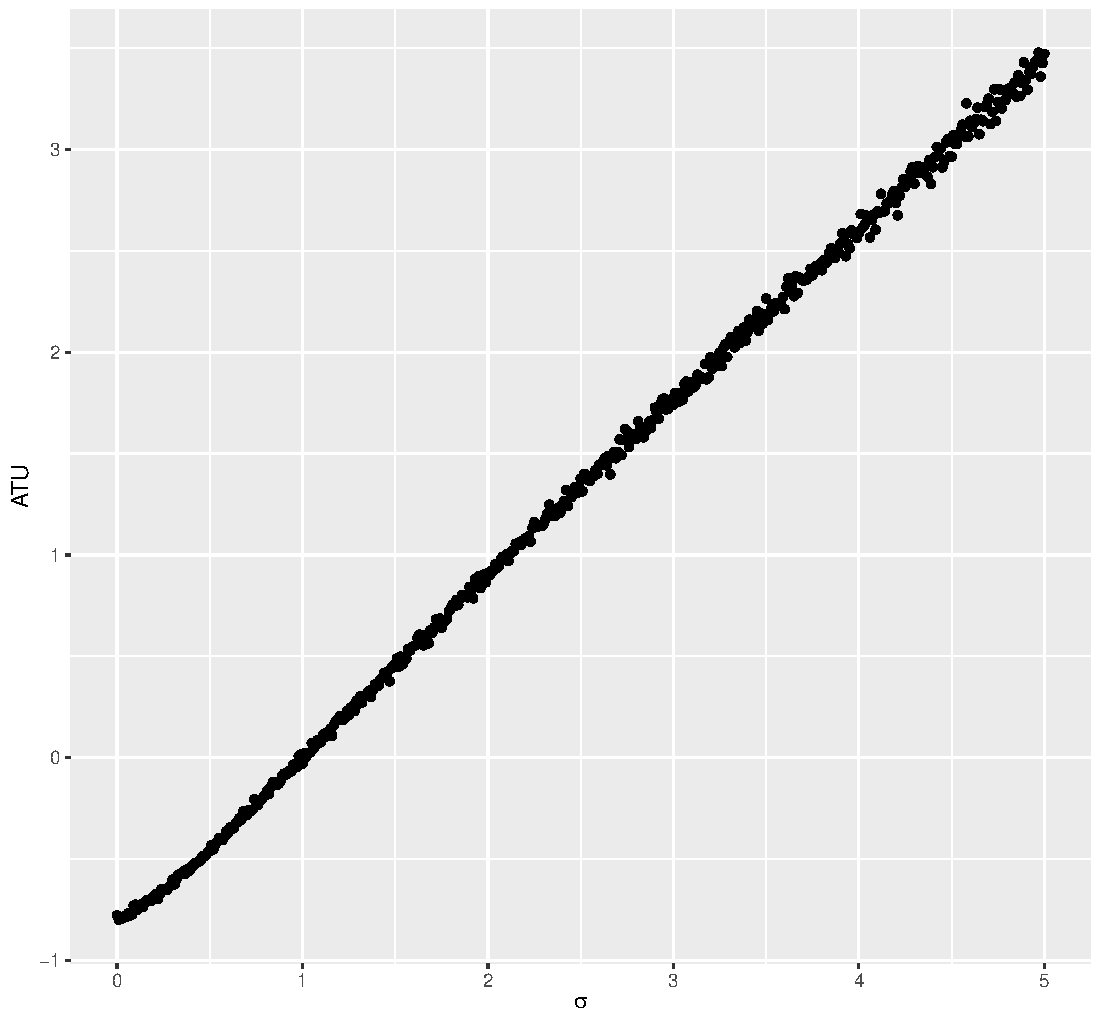
\includegraphics[width=0.43\textwidth]{ps1/Figures/p2_qe_beta.pdf}
    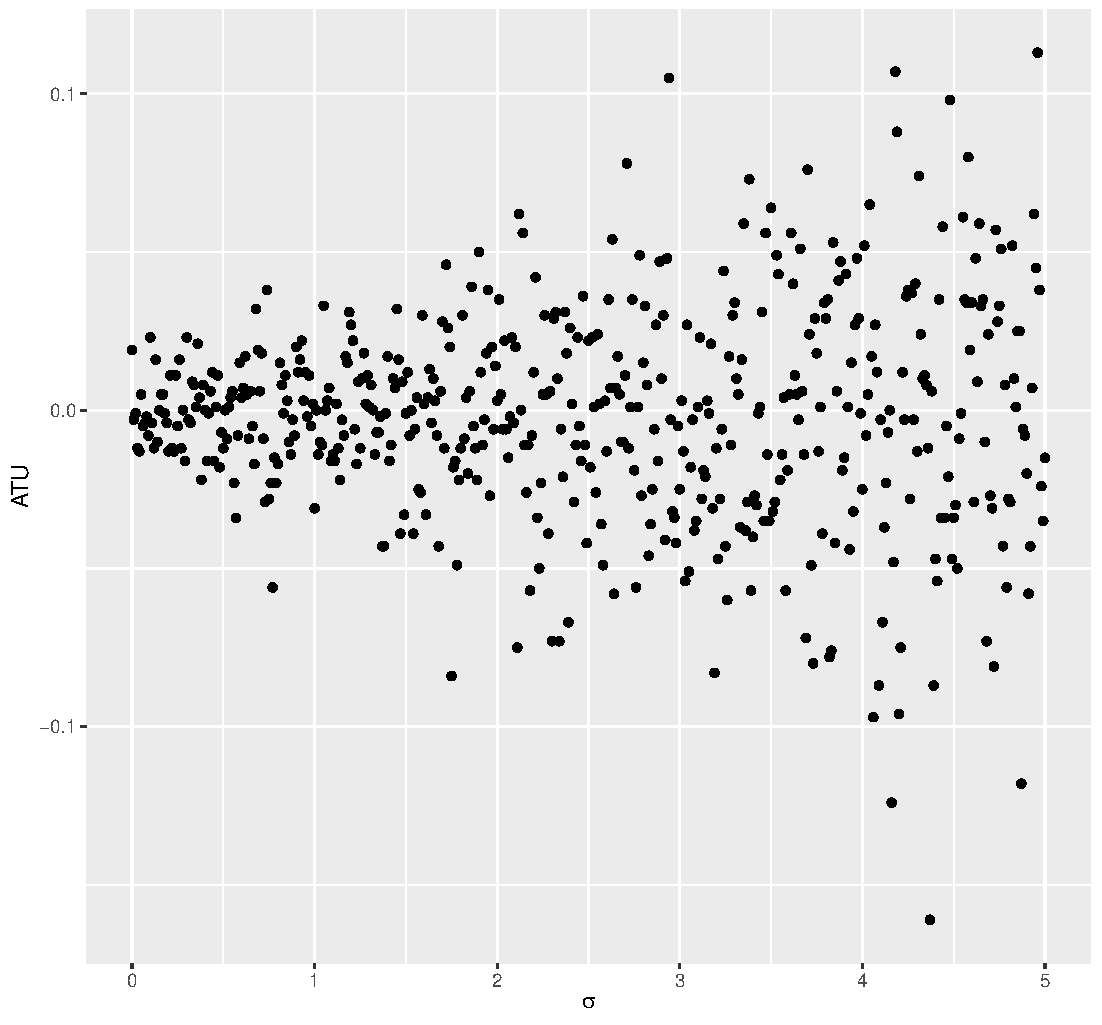
\includegraphics[width=0.43\textwidth]{ps1/Figures/p2_qe_ATE.pdf}
    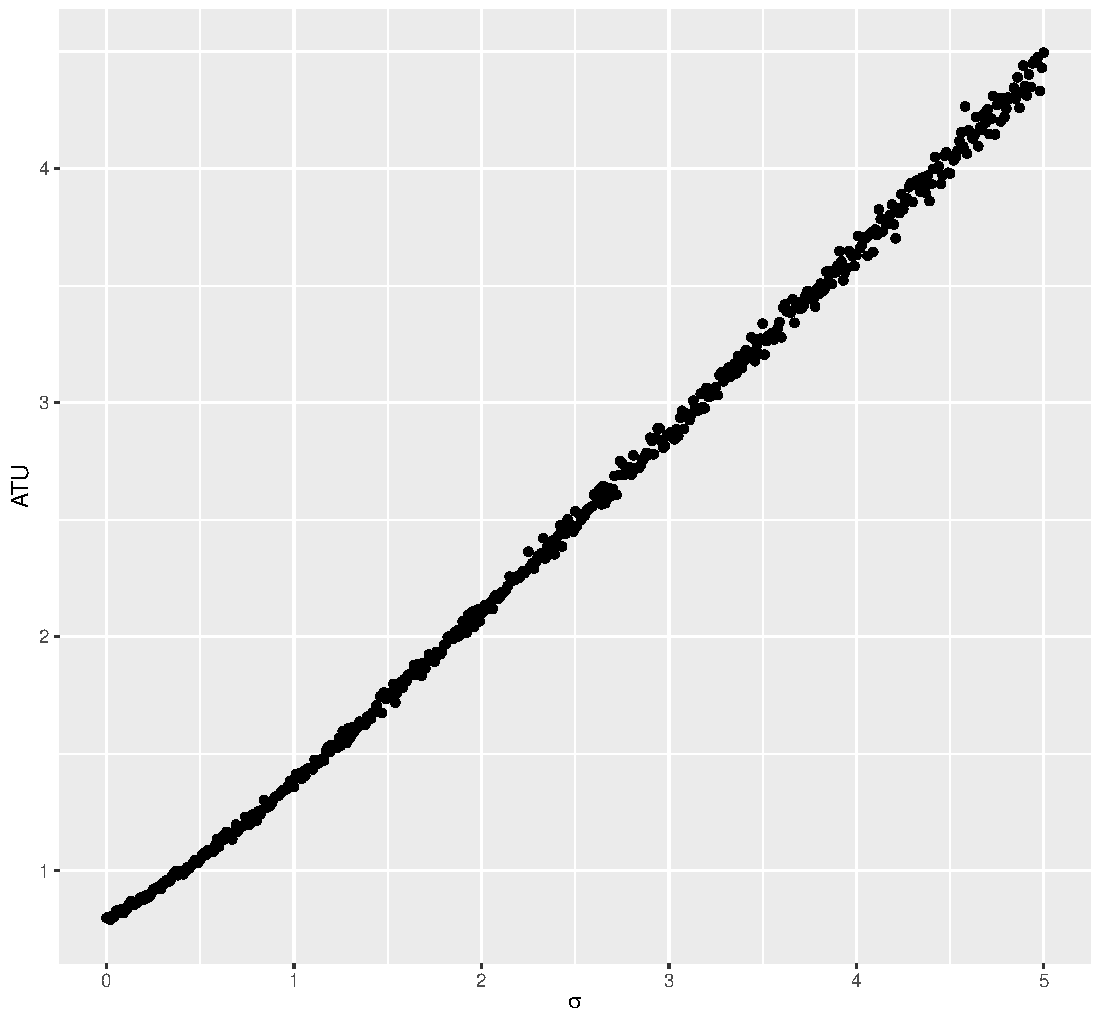
\includegraphics[width=0.43\textwidth]{ps1/Figures/p2_qe_ATT.pdf}
    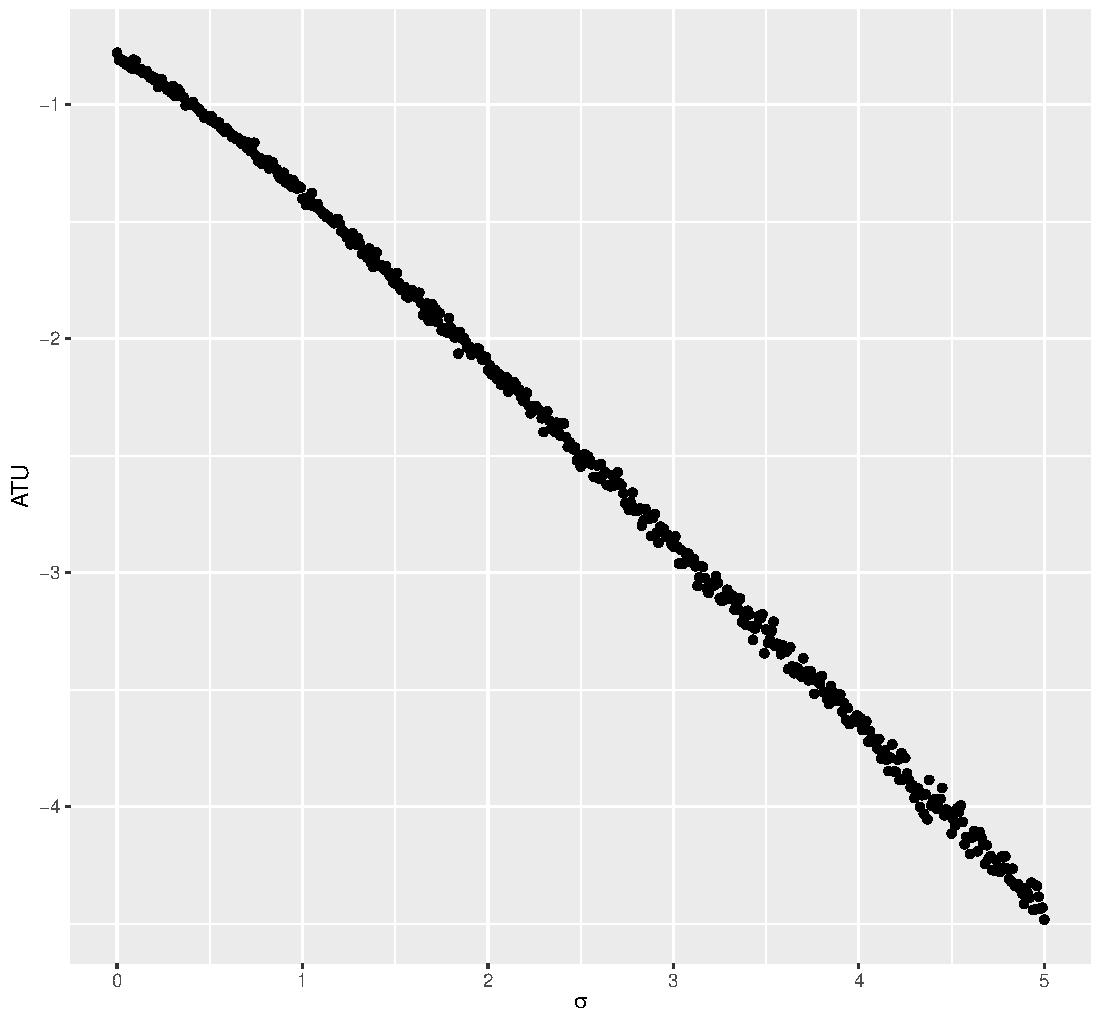
\includegraphics[width=0.43\textwidth]{ps1/Figures/p2_qe_ATU.pdf}
    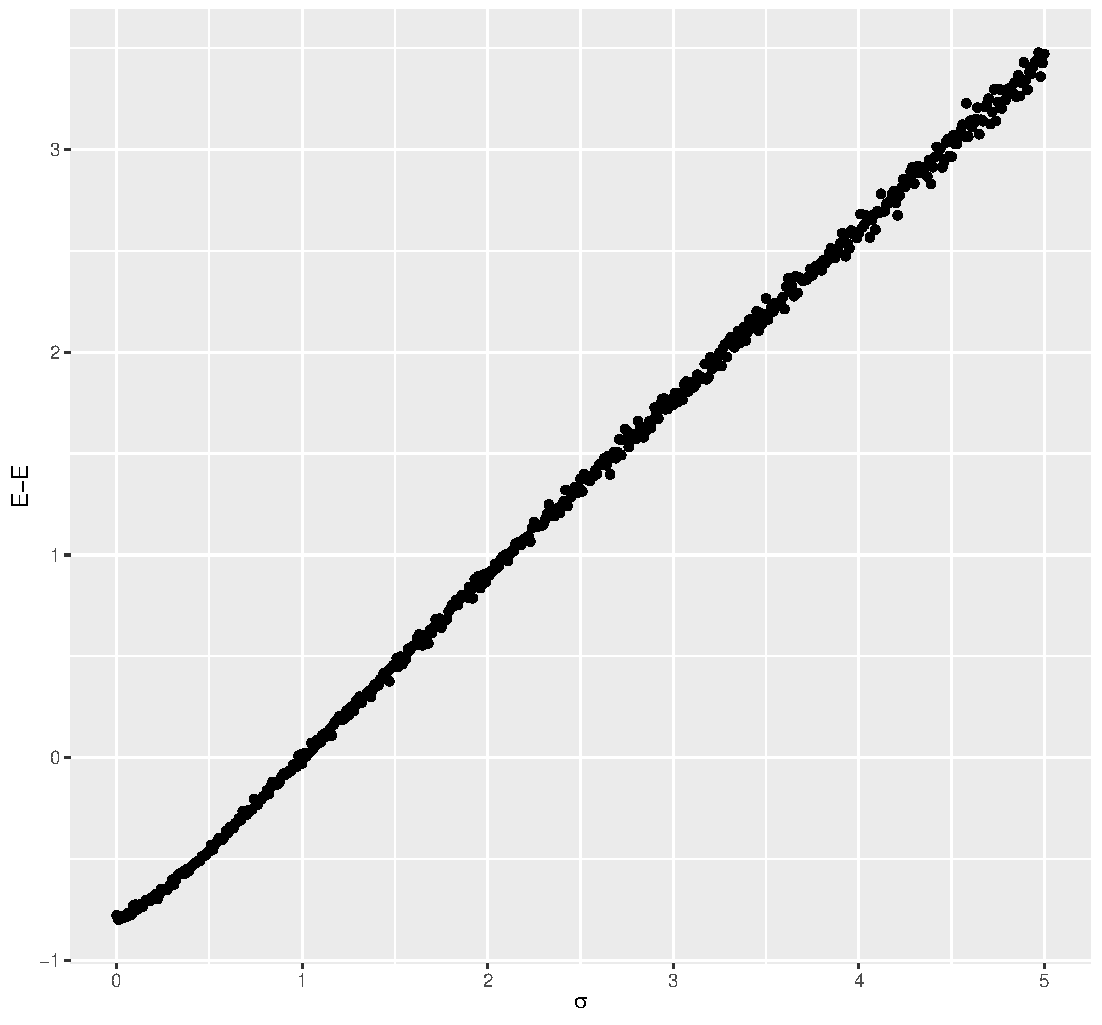
\includegraphics[width=0.43\textwidth]{ps1/Figures/p2_qe_param.pdf}
\end{figure}

\end{solution}
\begin{problem}{f}
Claim: in this setup, $D \perp\left(Y_{1}, Y_{0}\right)$ if and only if $\rho=0$. Argue whether this claim is true or not. Justify using the results from (e).
\end{problem}
\begin{solution}

\end{solution}


\newpage

%%%%%%%%%%%%%%%%%%%%%%%%%%%%%%%%%% QUESTION 3 %%%%%%%%%%%%%%%%%%%%%%%%%%%%%%%%%
\section*{Problem 3}
The purpose of this exercise is to introduce you to the bootstrapping procedure. In previous classes, you learned that, given i.i.d. data, the OLS estimator $\hat{\beta}$ will satisfy:
\begin{align*}
\hat{\beta} \stackrel{p}{\rightarrow} \beta=\mathbb{E}\left[X_{i} X_{i}^{\prime}\right]^{-1} \mathbb{E}\left[X_{i} Y_{i}\right] \quad \text { and } \quad \sqrt{N}(\hat{\beta}-\beta) \stackrel{d}{\rightarrow} \mathcal{N}(0, V),
\end{align*}
for some matrix $V$. Define $\hat{V}$ and $\operatorname{se}\left(\hat{\beta}_{k}\right)$ so that $\hat{V} \stackrel{p}{\rightarrow} V$ and $\operatorname{se}\left(\hat{\beta}_{k}\right)=\sqrt{\frac{1}{N} \operatorname{diag}(\hat{V})_{k}}$.
Monte Carlo Simulations
Consider the model $Y_{i}=X_{i}^{\prime} \beta+U_{i}$, where $U_{i} \mid X_{i} \stackrel{i . i . d}{\sim} \mathcal{N}\left(0, \sigma^{2}\right)$.
\begin{problem}{a}
Set $\beta=(2,3)^{\prime}$ and $\sigma^{2}=4$. Generate $N=10,000$ values for $X \in \mathbb{R}^{2}$ (one constant and one covariate). Given your value of $\sigma^{2}$, draw $U$ 's (they may be independent of $X$ ). Finally, compute $Y$ 's. Estimate $\hat{\beta}$ and its standard errors from your data using OLS.
\end{problem}
\begin{solution}
To see the full procedure see the attached code. The results presented in Table \ref{table:ea3:ps1:q3a:tab1}. These results are calculated using the OLS function from Matlab. However, the code fully calculates the point estimates and standard errors using the formulas and compares it to the estimates done by the build-in function. 
\begin{table}[htb]
\centering
\caption{OLS Estimates}
\label{table:ea3:ps1:q3a:tab1}
\begin{tabular}{lcccc}
\hline
 & Estimate & SE & tStat & pValue \\
\hline\hline
$\beta_0$ & 1.995 & 0.020 & 100.102 & 0.000 \\
$\beta_1$ & 3.004 & 0.020 & 150.589 & 0.000 \\
\hline
\end{tabular}
\end{table}

Note that the point estimates are almost identical to the true value. 
\end{solution}
\FloatBarrier
\begin{problem}{b}
Using $X, \beta$ and $\sigma^{2}$ from part (a), draw $S=10,000$ of $U^{(s)}$ (an $N \times 1$ vector for each $s$ ) and the corresponding $Y^{(s)}$. For each $Y^{(s)}$, compute the OLS estimator $\hat{\beta}^{(s)}$. Then, compute:
    \begin{align*}
        \sqrt{\widehat{\operatorname{Var}}\left[\hat{\beta}_{k}^{(s)} \mid X_{1}, \ldots, X_{N}\right]}=\sqrt{\frac{1}{S} \sum_{s=1}^{S}\left(\hat{\beta}_{k}^{(s)}\right)^{2}-\left(\frac{1}{S} \sum_{s=1}^{S} \hat{\beta}_{k}^{(s)}\right)^{2}} \stackrel{p}{\longrightarrow} \operatorname{se}\left(\hat{\beta}_{k} \mid X_{1}, \ldots, X_{N}\right)
    \end{align*}
    Justify the $" \stackrel{p}{\longrightarrow}$ " in the line above. Plot a histogram for the first component of $\beta^{(s)}$.
\end{problem}
\begin{solution}
For this problem it is important to highlight that $X$ is simulated from a standard normal distribution. The Monte Carlo estimation results are presented in Table \ref{table:ea3:ps1:q3a:tab2}. 
\begin{table}[htb]
\centering
\caption{Montecarlo Estimates}
\label{table:ea3:ps1:q3a:tab2}
\begin{tabular}{lcc}
\hline
 & Estimate & SE \\
\hline\hline
$\beta_0$ & 2.000 & 0.020 \\
$\beta_1$ & 3.001 & 0.020 \\
\hline
\end{tabular}
\end{table}
 \\ 
The Monte Carlo simulation cleans up some of the error induced by $U_i$ as our estimates are even closer to the true underlying value and the standard error is still the same. The convergence in probability of the estimated standard error to the theoretical is an application of both the Law of Large Numbers and the continuous mapping theorem. Each Monte Carlo estimated parameter $\hat{\beta}_k^{(s)}$ can be interpreted as a draw from the distribution of $\hat{\beta}_k$. Since $\hat{\beta}_k$ has a normal distribution then it has a second moment and 
\begin{align*}
    \frac{1}{S} \sum_{s=1}^{S}\left(\hat{\beta}_{k}^{(s)}\right)^{2}&\stackrel{p}{\longrightarrow}  \E[\hat{\beta}_k^2] & 
    \left(\frac{1}{S} \sum_{s=1}^{S} \hat{\beta}_{k}^{(s)}\right)^{2}&\stackrel{p}{\longrightarrow} \E[\hat{\beta}_k]^2
\end{align*}
by both the LLN and the continuous mapping theorem. To justify the claim that each $\hat{\beta}_k^{(s)}$ consider Figure \ref{ea3:ps1:q3a:fig1}. Note that over the 10,000 observations the implied histogram matches the pdf of the theoretical distribution. The theoretical distribution can be easily calculated as we selected $X_1\sim\mathcal{N}(0,1)$. Thus, the theoretical matrix $V$ is 
\begin{equation*}
    V = \E[X'X]\sigma^2 = \E\begin{bmatrix}
    1 & X_1 \\ X_1 & X_1^2
    \end{bmatrix}\sigma^2 = 
    \begin{bmatrix}
    4 & 0 \\ 0 & 4
    \end{bmatrix} 
\end{equation*}
Then for $N$ sufficiently large, the distribution of $\hat{\beta}$ is 
\begin{equation*}
    \hat{\beta}\sim\mathcal{N}\left(\begin{bmatrix}
    2 \\ 3
    \end{bmatrix},\begin{bmatrix}
    \sfrac{4}{N} & 0 \\ 0 & \sfrac{4}{N}
    \end{bmatrix}\right)
\end{equation*}
\begin{figure}[htb]
    \centering
    \caption{OLS Estimate Distribution from Montecarlo}
    \label{ea3:ps1:q3a:fig1}
    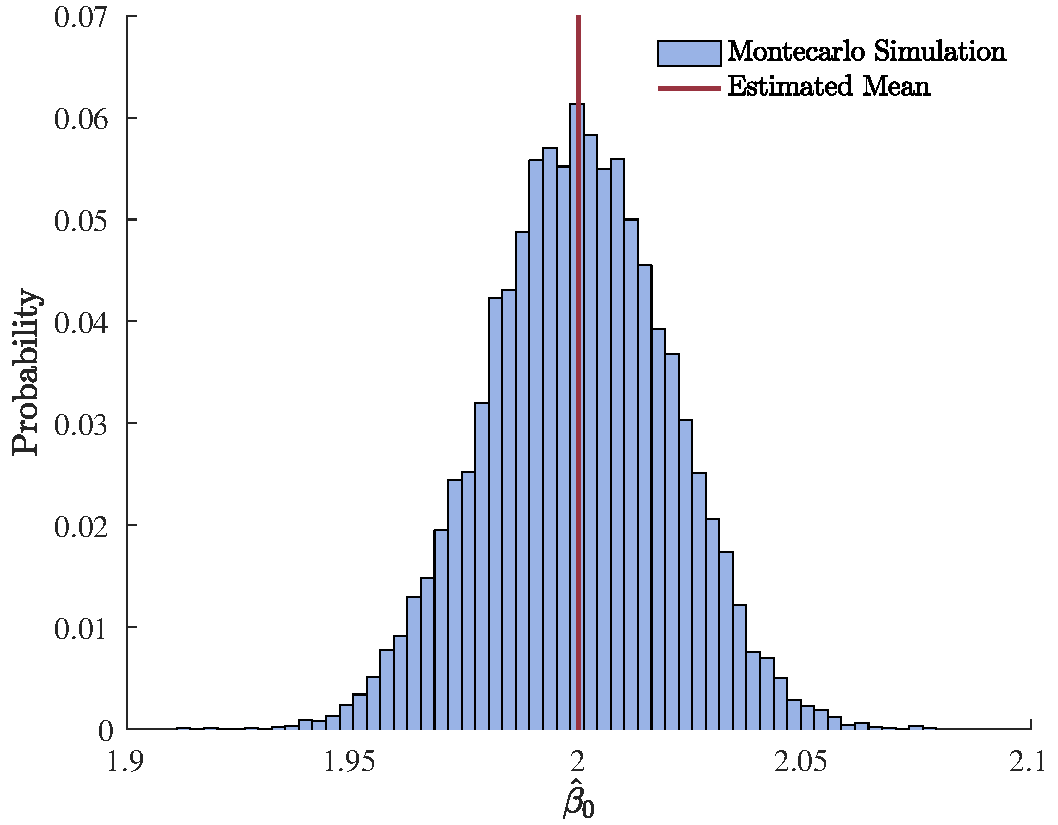
\includegraphics[width=0.43\textwidth]{Figures/p3qa.pdf}
\end{figure}

\end{solution}
\FloatBarrier
\underline{\hspace{\textwidth}}
\textbf{Nonparametric Bootstrap}
The rough idea behind bootstrapping is that we expect a large sample of observed data to behave like the wider population. Rather than drawing independent samples, which may be too costly or time-consuming, we can make inferences about our estimators by re-sampling from the original data. The rationale behind this idea is that the empirical distribution is close to the population distribution as the sample size becomes large. Through the bootstrap procedure, we can conduct inference about our estimates without specifying the data generating process. Consider the RCT setup: $Y=D Y_{1}+(1-D) Y_{0}$, where $D \perp\left(Y_{1}, Y_{0}\right)$.
\begin{problem}{a}
Define constant values for $Y_{1}=5+U_{1}$ and $Y_{0}=2+U_{2}$, where $U_{1}, U_{2} \stackrel{i . i . d}{\sim} N(0,1)$. Assign treatment $D \in\{0,1\}$ randomly (setting $P(D=1)=0.5$ is a good choice) to $N=10,000$ individuals. Estimate $E\left(Y_{1}-Y_{0}\right)$ using OLS and compute the standard errors. Then, argue that OLS gives consistent coefficient estimates. Why is $D \perp\left(Y_{1}, Y_{0}\right)$ important here?
\end{problem}
\begin{solution}
Begin by defining $Y$ to estimate the OLS regression as 
\begin{align*}
    Y   &= Y_1D + (1-D)Y_0 \\ 
        &= (Y_1-Y_0)D + Y_0
\end{align*}
By taking expectations it yields that 
\begin{equation*}
    \E[Y\vert D] = D\E[Y_1-Y_0\vert D] + \E[Y_0\vert D]
\end{equation*}
which implies that $\hat{\beta}_0=\E[Y_0\vert D] = \E[Y_0]$ using the independence assumption. Similarly, 
\begin{align*}
\hat{\beta}_1 & =\E[Y_1-Y_0\vert D] \\
&= \E[Y_1\vert D=1] - \E[Y_0\vert D=0] \\ 
&= \E[Y_1]-\E[Y_0] = \E[Y_1-Y_0] 
\end{align*}
But note that the independence assumption is key for the identification of the unconditional effect of the RCT. If $D\not\perp (Y_1,Y_0)$ then $\E[Y_1\vert D=1] - \E[Y_0\vert D=0]\neq \E[Y_1-Y_0]$. The results of the OLS regression are presented in Table \ref{table:ea3:ps1:q3b:tab1}.
\begin{table}[htb]
\centering
\caption{OLS Estimates}
\label{table:ea3:ps1:q3b:tab1}
\begin{tabular}{lcccc}
\hline
 & Estimate & SE & tStat & pValue \\
\hline\hline
$\beta_0$ & 2.000 & 0.014 & 139.305 & 0.000 \\
$\beta_1$ & 2.991 & 0.020 & 148.688 & 0.000 \\
\hline
\end{tabular}
\end{table}
 
Once again, the OLS results are close to the population value. 
\end{solution}
\begin{problem}{b}
From the initial data that you generated, draw $N=10,000$ pairs of $\left(Y_{i}, D_{i}\right)$, choosing each of the original data pairs with probability $\frac{1}{N}$ (with replacement). Repeat this procedure a total of $S=10,000$ times. You should have $S$ samples of $N=$ observations, each generated from the original sample. Repeat the computations from the Monte Carlo Simulations part, making sure to compute $\left(\widehat{\operatorname{Var}}\left[\hat{\beta}^{(s)}\right]\right)^{1 / 2}$ and to plot a histogram for $\hat{\beta}^{(s)}$. What would happen if you drew $Y$ and $D$ independently from the original sample, instead of as a pair?
\end{problem}
\begin{solution}
The results of the Bootstrap are presented in Table \ref{table:ea3:ps1:q3b:tab1}. One key feature of the Bootstrap exercise is that the distribution generated by Bootstrapping is not the theoretical one but in reality the distribution around the OLS estimates. 
\begin{table}[htb]
\centering
\caption{Bootstrap Estimates}
\label{table:ea3:ps1:q3b:tab2}
\begin{tabular}{lcc}
\hline
 & Estimate & SE \\
\hline\hline
$\beta_0$ & 2.008 & 0.014 \\
$\beta_1$ & 2.978 & 0.020 \\
\hline
\end{tabular}
\end{table}

To see this clearly, refer to Figure \ref{ea3:ps1:q3b:fig1}. The Empirical distribution is constructed using a normal distribution center around the OLS estimate and the variance is the square of the estimated standard error calculated by OLS. 
\begin{figure}[htb]
    \centering
    \caption{OLS Estimate Distribution from Bootstrapping}
    \label{ea3:ps1:q3b:fig1}
    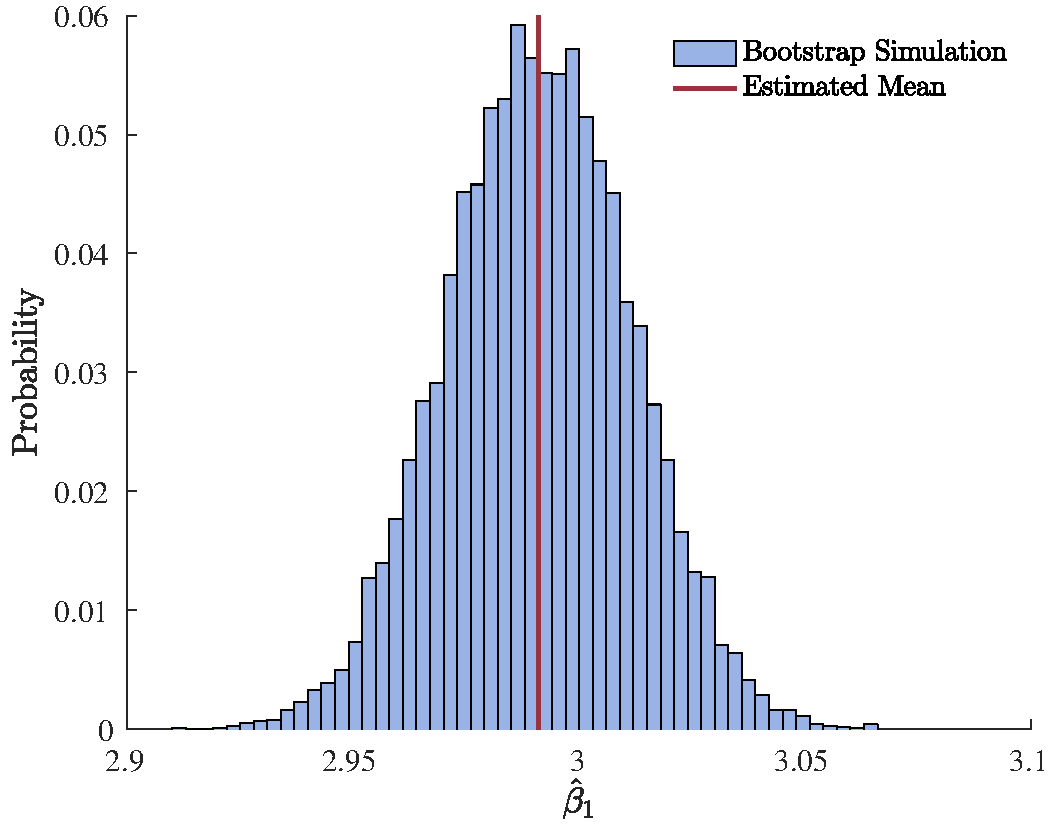
\includegraphics[width=0.43\textwidth]{Figures/p3qb.pdf}
\end{figure}
\end{solution}
\end{document}
